\documentclass[24pt,pdf,hyperref={unicode},aspectratio=169]{beamer}
\usepackage[utf8]{inputenc}
\usepackage{aiml}

\begin{document}


\section{Карты Кохонена}

\begin{frame}\frametitle{Обучение без учителя}
\begin{center}
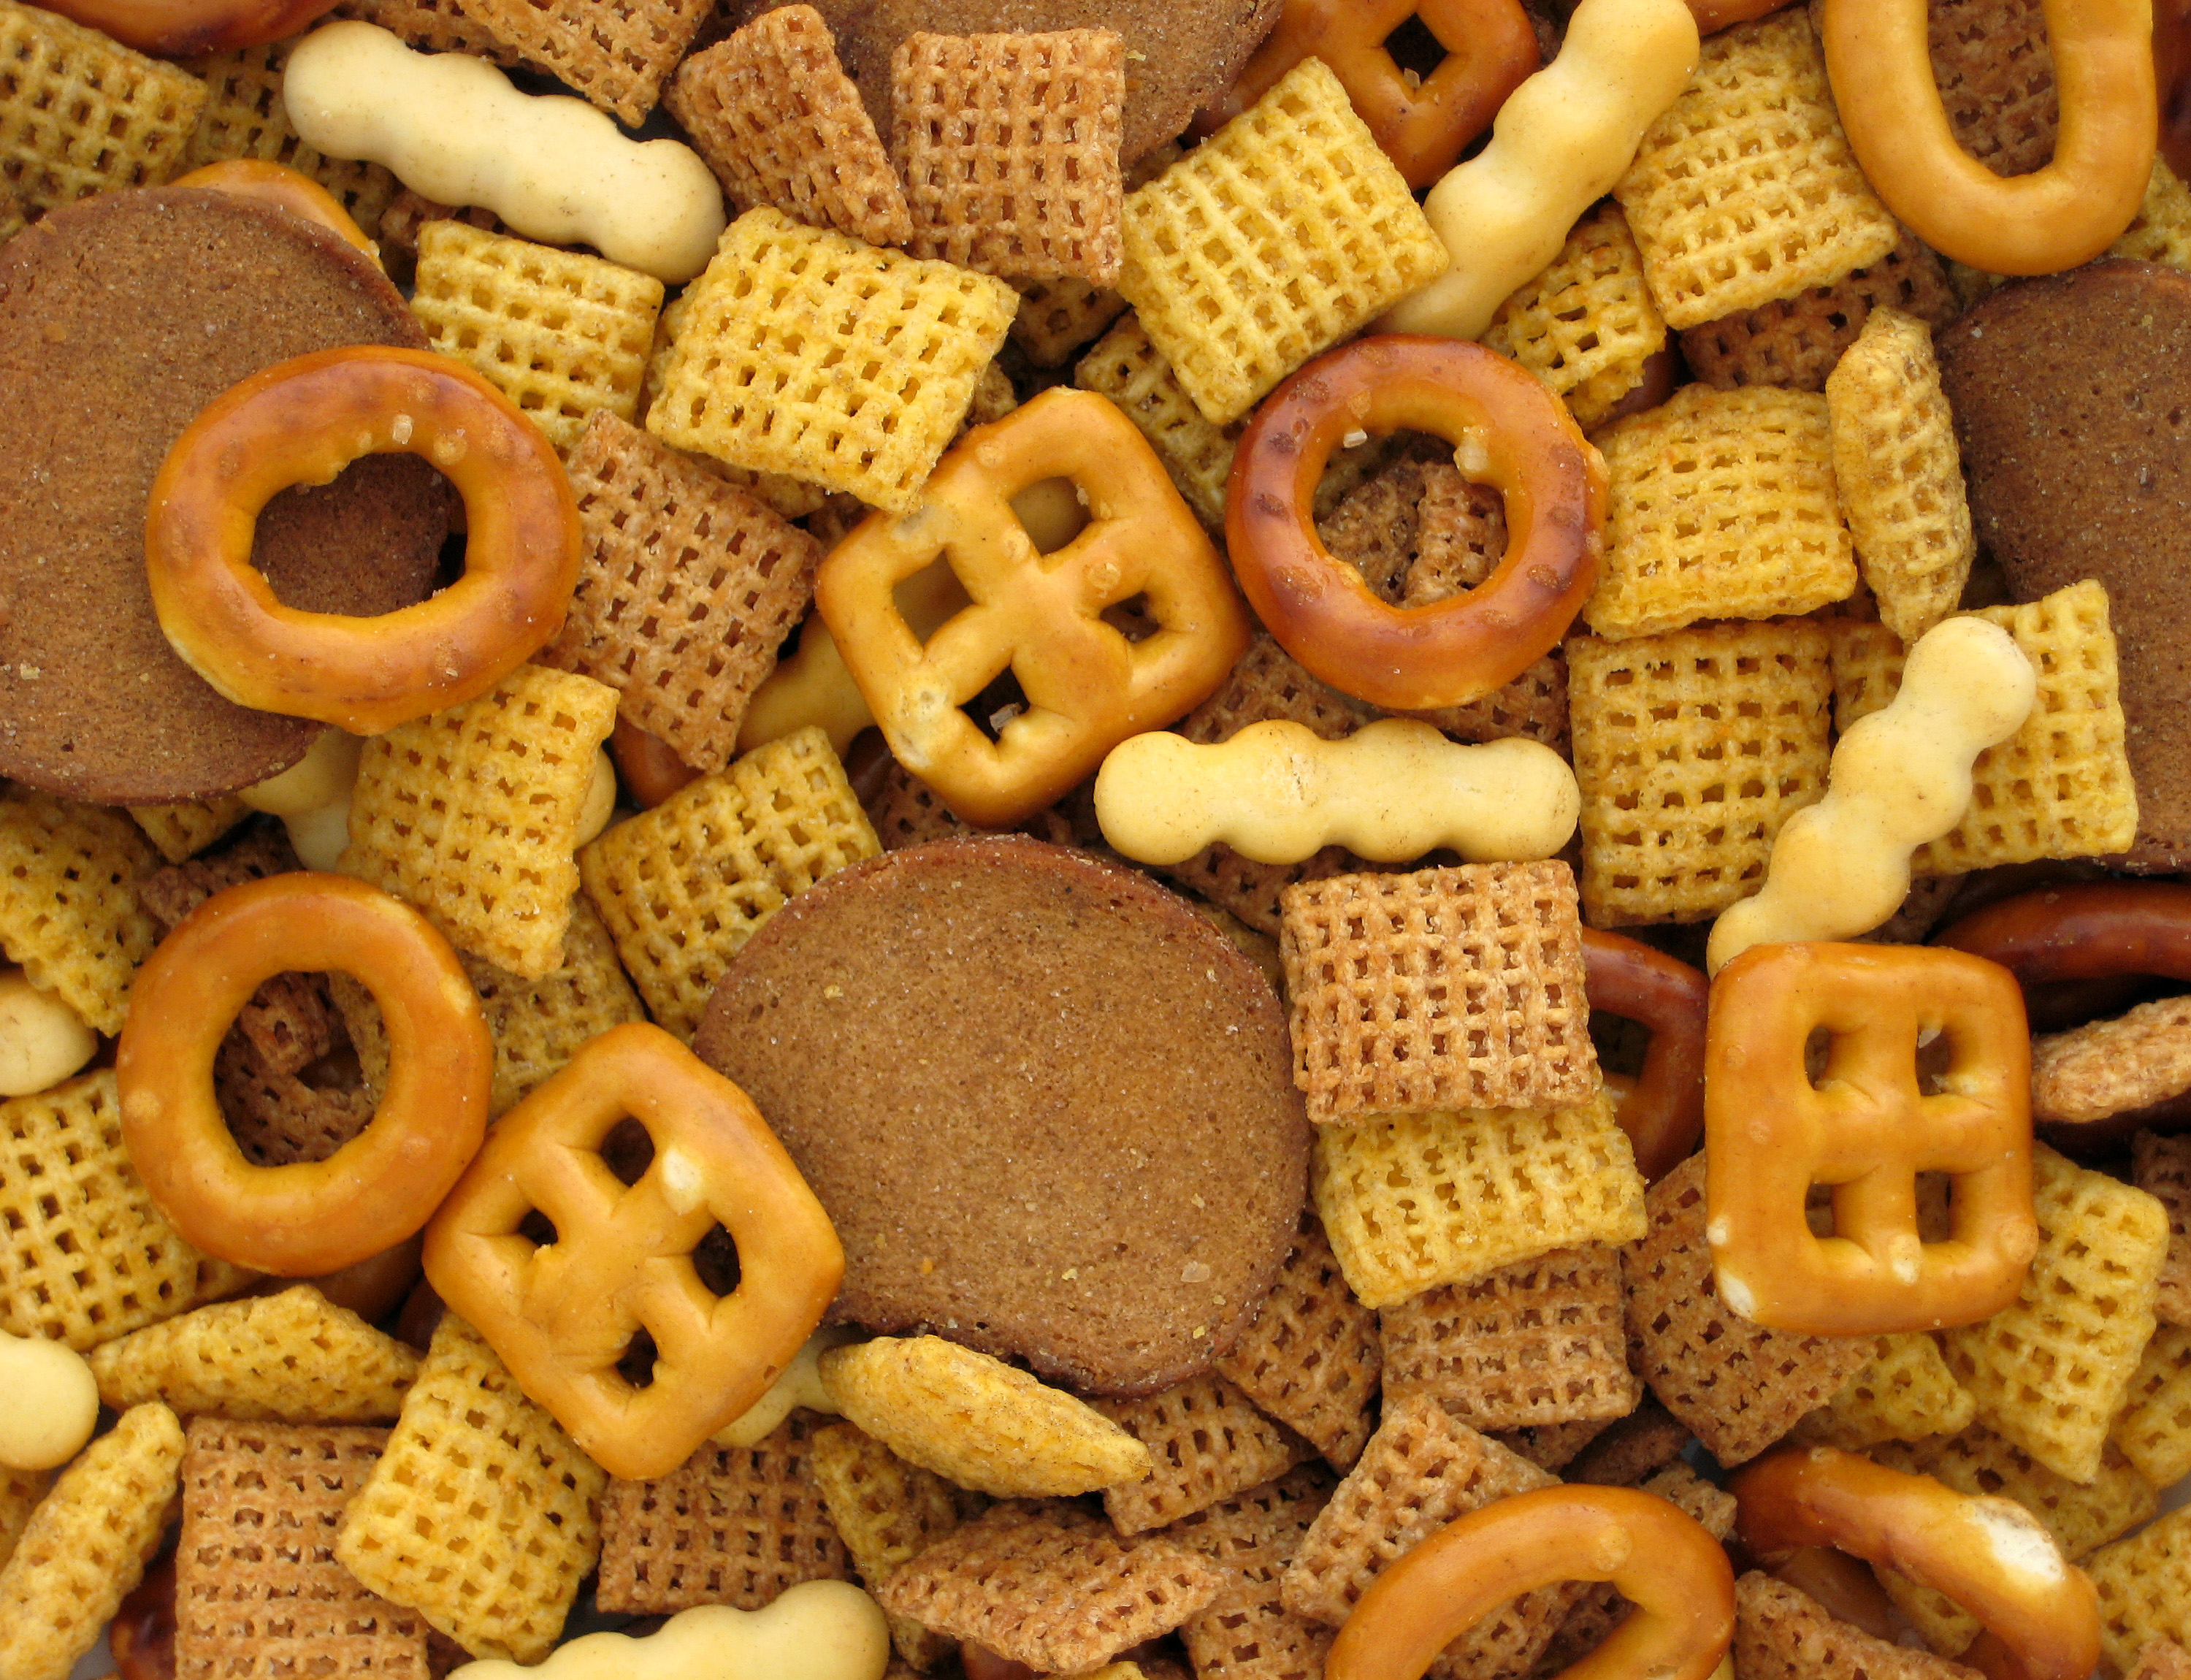
\includegraphics[width=0.7\textwidth]{Images/cookies.jpg}
\end{center}
\end{frame}

\begin{frame}\frametitle{Обучение без учителя}
\begin{center}
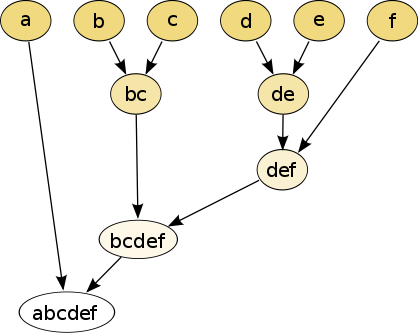
\includegraphics[width=0.5\textwidth]{Images/dendrogramm.png}
\end{center}
\end{frame}


\usetikzlibrary{calc}

\begin{frame}\frametitle{Карты Кохонена}
\begin{columns}

\column{0.4\textwidth}
\begin{tikzpicture}
\foreach \x in {1,...,5}
\foreach \y in {1,...,4}
{
\draw (\x,\y) -- ($(\x,\y)+(0,1)$);
\draw (\y,\x) -- ($(\y,\x)+(1,0)$);
}

\foreach \x in {1,...,5}
\foreach \y in {1,...,5}
{
\node[circle,draw=black,fill=white,inner sep=0cm] (n-\x-\y) at (\x,\y) {$N_{\x,\y}$};
}

\end{tikzpicture}

\column{0.6\textwidth}
\uncover<+->{}
\uncover<+->{$$
W_{i,j}\in\mathbb{R}^n
$$}
\uncover<+->{$$
X\in\mathbb{R}^n
$$}
\uncover<+->{$$
X\rightarrow \ (i,j)\ :\ ||W_{i,j}-X||=\min
$$}
\uncover<+->{$$
W'_{i,j}=(1-\varepsilon) W_{i,j}+\varepsilon X
$$}
\uncover<+->{$$
\varepsilon_{k,l}=\varepsilon c^{|k-i|+|l-j|}
$$}
\uncover<+->{$$
W'_{k,l}=(1-\varepsilon_{k,l}) W_{k,l}+\varepsilon_{k,l} X
$$}
\end{columns}

\end{frame}


\end{document}